\documentclass[a4paper, 12pt, projekat]{etf}
\usepackage[intlimits]{amsmath}
\usepackage{amsmath, amsfonts, amssymb, graphicx}
\usepackage[serbian]{babel}
\usepackage[T1]{fontenc}
\usepackage[utf8]{inputenc}
\usepackage{dirtree}
\addto\captionsserbian{%
	\renewcommand{\bibname}%
	{Literatura}%
}


\title{Simulacija zagušenja pomoću ns-3}
\author{Aleksandar Popović}
\indeks{2020/0059}
\date{jul 2023.}
\mentor{prof. dr Milan Bjelica}
\predmet{Primena modernih telekomunikacija}

\begin{document}
	\maketitle
	\begin{abstract}
		U ovom radu je pomoću simulatora NS-3 pokazano kako zagušenje mreže utiče na propusnost saobraćaja. Simulirana je mreža od četiri računara, međusobno povezanih u topologiju zvezde gde dva računara tokom trajanja simulacije generišu saobraćaj ka trećem. Loša propusnost je pokazana velikim brojem odbačenih paketa. Posle se mreža poboljšava tako što se proširi kapacitet linka koji je usko grlo i napravi se poređenje rezultata.
	\end{abstract}
	\begin{keywords}
		ns-3, simulacija, zagu\v{s}enje
	\end{keywords}
	\tableofcontents
	\listoffigures
	\listoftables
	
	\chapter{Uvod}
	U ovom radu će se obraditi simulacija zagušenja mreže pomoću simulatora NS-3(Network Simulator 3). 
	Simulator je slobodan softver; njegov izvorni kod je javno dostupan za proučavanje i izmenu.
	
	
	U simulaciji će se pokazati kako preopterećenje veze dovodi do gubitaka paketa i kako se performanse poboljšavaju posle povećanja kapaciteta linka.
	
	
	U nastavku će biti opisan postupak pokretanja simulacije, opis simulirane topologije i pregled rezultata.
	
	\chapter{Opis simulacije}
	
	\section{Opis mreže}
	Topologija simulirane mreže je predstavljena na slici \ref{fig:topologija}. Mreža se sastoji od četiri računara koja su povezana PPP (\emph{Point to Point Protocol}) vezama. Na računarima označenim brojevima 2 i 3 su instalirane aplikacije koje šalju UDP (\emph{User Datagram Protocol}) pakete ka računaru označenim brojem 0. 
	\begin{figure}[htb]
		\centering
		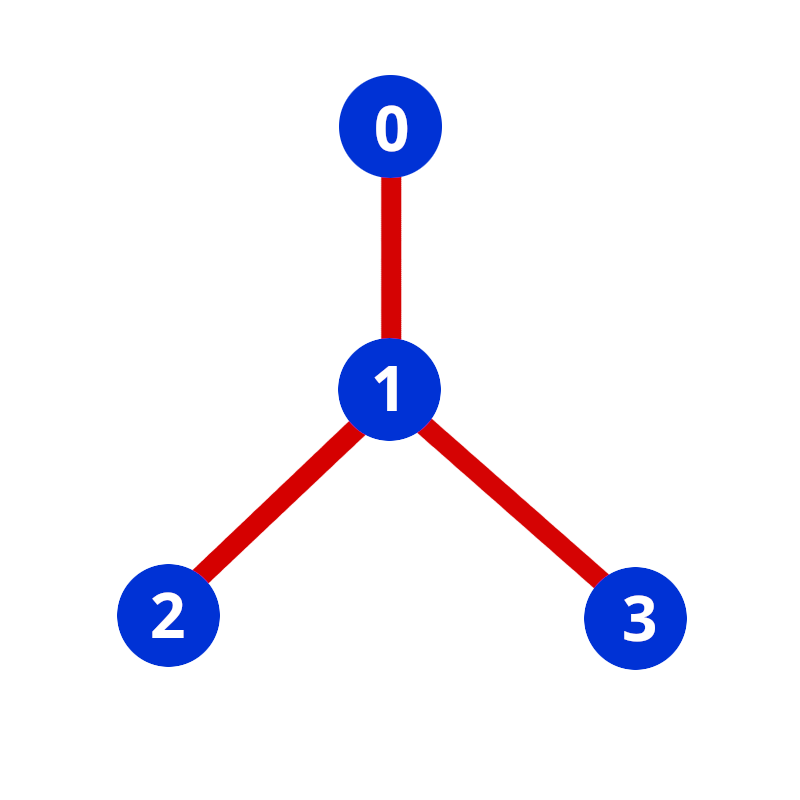
\includegraphics[width=.6\textwidth]{../slike/topologija.png}
		\caption{\emph{Topologija}}
		\label{fig:topologija}
	\end{figure}
	
	Prvobitno su kapaciteti svih linkova isti i iznose 1\! Mbps.  Aplikacije konstantno šalju pakete veličine 200\! b brzinom od 5000 paketa u sekundi. Tako se prouzrokuje zagušenje saobraćaja u mrežnom uređaju u računaru 0 koji se manifestuje gubitkom paketa. Potom se kapacitet linka poveća na 10\! Mbps i posmatra se kako su se promenile performanse mreže.\\
	IP adrese dodeljene mrežnim uređajima su navedene u tabeli \ref{tab:adr}
	\begin{table}[htb]
		\centering
		\caption{Adrese mrežnih uređaja}
		\label{tab:adr}
		\medskip
		\begin{tabular}{c|r}
			\hline
			Mrežni uređaj & Adresa \\
			\hline
			0 & 10.0.0.2 \\
			1 & 10.0.0.1 \\
			2 & 10.0.1.2 \\
			3 & 10.0.1.1 \\
			4 & 10.0.2.2 \\
			5 & 10.0.2.1
		\end{tabular}
	\end{table}
	
	\section{Pokretanje simulacije}
	\subsection{Preduslovi}
	Simulator je potrebno instalirati na \emph{Linux} operativnom sistemu pri\-drža\-vajući se zvaničnog uputstva. \cite{ns3man} Posle instalacije je potrebno napraviti promenljivu okruženja \verb|NS3ROOT| koja će imati vrednost putanje do korena NS-3 simulatora pokretanjem sledeće komande u terminalu:\\
	
	
	\verb|$ NS3ROOT=putanja_do_direktorijuma|\\
	
	Pošto je doseg ove promenljive vezan za sam proces terminala, preporučuje se da se na kraj fajla \verb|~/.bashrc| doda linija:\\
	
	\verb|export NS3ROOT=putanja_do_direktorijuma|\\
	
	Tako će i prilikom ponovnog pokretanja sistema biti definisana ova promenljiva.
	
	\subsection{Pokretanje skripte}
	U direktorijumu projekta se nalazi \emph{Bash} skripta \verb|run.sh|. Potrebno ju je korišćenjem terminala učiniti izvršivom i pokrenuti je na sledeći način:
	\begin{verbatim}
		$ chmod u+x run.sh
		$ ./run.sh
	\end{verbatim}
	
	
	Skripta radi tako što sve fajlove iz \verb|h/| i \verb|src/| direktorijuma projekta kopira u \verb|scratch/| direktorijum simulatora. Posle kopiranja pokreće kompilaciju i izlazne fajlove snima \verb|output/| direktorijum. U \verb|output/| direktorijumu će se pojaviti dva izlazna XML fajla u kojima će se naći broj odbačenih paketa na svakom mrežnom uređaju.
	
	\section{Opis skripte}
	Glavni deo skripte je u funkciji \verb|void buildTopology(bool optimize)| koja u zavisnosti od parametra pravi mrežu u kojoj je link između računara 0 i 1 kapaciteta 1\! Mbps ili 10\! Mbps.
	\subsection{Kreiranje uređaja i veza između njih}
	\begin{verbatim}
		NodeContainer nodes;
		nodes.Create(4);
		
		InternetStackHelper internet;
		internet.Install(nodes);
		
		PointToPointHelper p2p;
		p2p.SetQueue("ns3::DropTailQueue",
		    "MaxSize", StringValue(QueueSize));
		p2p.SetDeviceAttribute("DataRate", 
		    StringValue(BaseBandwidth));
		p2p.SetChannelAttribute("Delay", StringValue(LinkDelay));
		NetDeviceContainer n2n1 = p2p.Install(nodes.Get(2), 
		    nodes.Get(1));
		NetDeviceContainer n3n1 = p2p.Install(nodes.Get(3), 
		    nodes.Get(1));
		if(optimize){
			p2p.SetDeviceAttribute("DataRate", 
			    StringValue(IncreasedBandwidth));
		}
		NetDeviceContainer n1n0 = p2p.Install(nodes.Get(1),
		    nodes.Get(0));
	\end{verbatim}
	
	Možemo primetiti da će veza između računara 0 i 1 biti povećanog ka\-pa\-citeta ako parametar \verb|optimize| ima vrednost \verb|true|.
	\subsection{Dodela adresa}
	U ovom delu skripte će se mrežnim uređajima dodeliti IP adrese i po\-puniće se tabele rutiranja.
	\begin{verbatim}
	Ipv4AddressHelper ip;
	
	ip.SetBase("10.0.0.0", "255.255.255.0");
	Ipv4InterfaceContainer i1i0 = ip.Assign(n1n0);
	
	ip.SetBase("10.0.1.0", "255.255.255.0");
	Ipv4InterfaceContainer i2i1 = ip.Assign(n2n1);
	
	ip.SetBase("10.0.2.0", "255.255.255.0");
	Ipv4InterfaceContainer i3i1 = ip.Assign(n3n1);
	
	Ipv4GlobalRoutingHelper::PopulateRoutingTables();
	\end{verbatim}
	\subsection{Izvor saobraćaja}
	Na računarima 2 i 3 su instalirane aplikacije koje šalju UDP pakete ka računaru 0. Aplikacije će biti pokrenute u trajanju od 20 sekundi.
	\begin{verbatim}
		uint16_t port = 9;
		OnOffHelper sender("ns3::UdpSocketFactory",
		    InetSocketAddress(i1i0.GetAddress(1),port));
		sender.SetAttribute("OnTime", 
		    StringValue("ns3::ConstantRandomVariable[Constant=1]"));
		sender.SetAttribute("OffTime", 
		    StringValue("ns3::ConstantRandomVariable[Constant=0]"));
		sender.SetAttribute("DataRate", StringValue(BaseBandwidth));
		sender.SetAttribute("PacketSize", UintegerValue(200));
		ApplicationContainer senderApps = 
		    sender.Install(NodeContainer(nodes.Get(2), nodes.Get(3)));
		senderApps.Start(Seconds(0.0));
		senderApps.Stop(Seconds(20.0));
	\end{verbatim}
	\subsection{Prijem saobraćaja}
	Aplikacija za prijem saobraćaja na računaru 0 će biti aktivna 10 sekundi duže zbog eventualnih paketa u redovima čekanja na slanje.
	\begin{verbatim}
		PacketSinkHelper sink("ns3::UdpSocketFactory",
		    InetSocketAddress(Ipv4Address::GetAny(),port));
		ApplicationContainer sinkApps = sink.Install(nodes.Get(0));
		sinkApps.Start(Seconds(0.0));
		sinkApps.Stop(Seconds(30.0));
	\end{verbatim}
	\subsection{Izvršavanje simulacije i snimanje izveštaja}
	Za analizu simulacije je upotrebljena \verb|ns3::FlowMonitor| klasa čiji opis je dostupan u dokumentaciji.\cite{ns3doc}
	\begin{verbatim}
		Ptr<FlowMonitor> flowMonitor;
		FlowMonitorHelper flowMonitorHelper;
		flowMonitor = flowMonitorHelper.InstallAll();
		
		Simulator::Stop(Seconds(30.0));
		Simulator::Run();
		
		flowMonitor->SerializeToXmlFile
		    (optimize?"izlazsa.xml":"izlazbez.xml", false,true);
		Simulator::Destroy();
	\end{verbatim}
	
	
	\chapter{Rezultati}
	U tabeli \ref{tab:pakpre} su prikazani rezultati simulacije pre optimizacije, a u tabeli \ref{tab:pakposle} posle optimizacije
	\begin{table}[htb]
		\centering
		\caption{Pre optimizacije}
		\label{tab:pakpre}
		\medskip
		\begin{tabular}{l|r}
			\hline
			Poslato paketa & 24998 \\
			Primljeno paketa & 13144 \\
			Izgubljeno paketa & 11854 \\
		\end{tabular}
	\end{table}
	\begin{table}[htb]
		\centering
		\caption{Posle optimizacije}
		\label{tab:pakposle}
		\medskip
		\begin{tabular}{l|r}
			\hline
			Poslato paketa & 24998 \\
			Primljeno paketa & 23808 \\
			Izgubljeno paketa & 1190 
		\end{tabular}
	\end{table}
	
	Rezultati su pokazali da je zbog uskog grla drastično smanjen kvalitet saobraćaja. Posle optimizacije je procenat izgubljenih paketa smanjen sa $47.42\%$ na $4.76\%$.
	
	\chapter{Zaključak}
	U ovom projektu je prikazana simulacija zagušenja korišćenjem NS-3 simulatora. Opisana je mreža u kojoj je zagušenje pokazano i objašnjena je skripta  kojom je simulacija kreirana. Pokazano je kako nedovoljan kapacitet linka negativno utiče na kvalitet saobraćaja. Topologija je relativno jednostavna jer cilj rada nije bila kompleksnost, nego pokazivanje mogućnosti analize mreže uz pomoć simulatora. 
	\begin{thebibliography}{10}
		\addcontentsline{toc}{chapter}{Literatura}
		\bibitem{ns3man} \emph{ns-3 Tutuorial}, izdanje za ns-3.38, 2023; dostupno online:
		https://www.nsnam.org/docs/release/3.38/tutorial/ns-3-tutorial.pdf
		\bibitem{ns3doc} ns-3 dokumentacija: https://www.nsnam.org/docs/doxygen/index.html
 	\end{thebibliography}
 	
	\chapter*{Prilozi} \addcontentsline{toc}{chapter}{Prilozi}
	\section*{Struktura direktorijuma projekta}\addcontentsline{toc}{section}{Struktura direktorijuma projekta}
	\dirtree{%
		.1 pmt-projekat/. 
		.2 run.sh. 
		.2 h/. 
		.3 topology.h. 
		.2 src/. 
		.3 main.cc.
		.3 topology.cc.	
		.2 output/. 	
	}
	\section*{\emph{run.sh}}\addcontentsline{toc}{section}{\emph{run.sh}}
	\begin{verbatim}
		#!/bin/bash
		
		mkdir -p "$NS3ROOT/scratch/projekat"
		
		pushd src
		for file in $(ls)
		do
		cp $file "$NS3ROOT/scratch/projekat/$file"
		done
		popd
		
		pushd h
		for file in $(ls)
		do
		cp $file "$NS3ROOT/scratch/projekat/$file"
		done
		popd
		
		mkdir -p output
		OUTDIR="$PWD/output"
		
		pushd "$NS3ROOT"
		./ns3 build
		./ns3 run scratch/projekat/main.cc --cwd=$OUTDIR
		popd
		
	\end{verbatim}
	\section*{\emph{topology.h}}\addcontentsline{toc}{section}{\emph{topology.h}}
	\begin{verbatim}
		#pragma once
		#include <iostream>
		#include <fstream>
		#include <string>
		#include <cassert>
		
		#include "ns3/core-module.h"
		#include "ns3/internet-module.h"
		#include "ns3/point-to-point-module.h"
		#include "ns3/network-module.h"
		#include "ns3/applications-module.h"
		#include "ns3/ipv4-global-routing-helper.h"
		#include "ns3/flow-monitor.h"
		#include "ns3/flow-monitor-helper.h"
		
		#define BaseBandwidth "1Mbps"
		#define IncreasedBandwidth "10Mbps"
		#define QueueSize "1024p"
		#define LinkDelaz "5ms"
		
		
		using namespace ns3;
		
		void buildTopology(bool optimize);
	\end{verbatim}
	\section*{\emph{topology.cc}}\addcontentsline{toc}{section}{\emph{topology.cc}}
	\begin{verbatim}
		#include "topology.h"
		
		void buildTopology(bool optimize){
			NodeContainer nodes;
			nodes.Create(4);
			
			//instalacija steka protokola na cvorovima
			InternetStackHelper internet;
			internet.Install(nodes);
			
			//pravimo linkove
			PointToPointHelper p2p;
			p2p.SetQueue("ns3::DropTailQueue", 
			    "MaxSize", StringValue(QueueSize));
			p2p.SetDeviceAttribute("DataRate", 
			    StringValue(BaseBandwidth));
			p2p.SetChannelAttribute("Delay", StringValue(LinkDelay));
			NetDeviceContainer n2n1 = p2p.Install
			    (nodes.Get(2), nodes.Get(1));
			NetDeviceContainer n3n1 = p2p.Install
			    (nodes.Get(3), nodes.Get(1));
			if(optimize){
				p2p.SetDeviceAttribute("DataRate",
				    StringValue(IncreasedBandwidth));
			}
			NetDeviceContainer n1n0 = 
			    p2p.Install(nodes.Get(1), nodes.Get(0));
			
			//dodela IP adresa
			Ipv4AddressHelper ip;
			
			ip.SetBase("10.0.0.0", "255.255.255.0");
			Ipv4InterfaceContainer i1i0 = ip.Assign(n1n0);
			
			ip.SetBase("10.0.1.0", "255.255.255.0");
			Ipv4InterfaceContainer i2i1 = ip.Assign(n2n1);
			
			ip.SetBase("10.0.2.0", "255.255.255.0");
			Ipv4InterfaceContainer i3i1 = ip.Assign(n3n1);
			
			Ipv4GlobalRoutingHelper::PopulateRoutingTables();
			
			//izvor saobracaja
			uint16_t port = 9;
			OnOffHelper sender("ns3::UdpSocketFactory", 
			    InetSocketAddress(i1i0.GetAddress(1),port));
			sender.SetAttribute("OnTime", 
			    StringValue("ns3::ConstantRandomVariable[Constant=1]"));
			sender.SetAttribute("OffTime", 
			    StringValue("ns3::ConstantRandomVariable[Constant=0]"));
			sender.SetAttribute("DataRate", StringValue(BaseBandwidth));
			sender.SetAttribute("PacketSize", UintegerValue(200));
			ApplicationContainer senderApps = 
			    sender.Install(NodeContainer(nodes.Get(2), nodes.Get(3)));
			senderApps.Start(Seconds(0.0));
			senderApps.Stop(Seconds(20.0));
			
			//prijem saobracaja
			PacketSinkHelper sink("ns3::UdpSocketFactory",
			    InetSocketAddress(Ipv4Address::GetAny(),port));
			ApplicationContainer sinkApps = sink.Install(nodes.Get(0));
			sinkApps.Start(Seconds(0.0));
			sinkApps.Stop(Seconds(30.0));
			
			
			//snimanje izvestaja
			AsciiTraceHelper ascii;
			Ptr<OutputStreamWrapper> stream = ascii.CreateFileStream
			    (optimize?"bezoptimizacije.tr":"saoptimizacijom.tr");
			p2p.EnableAsciiAll(stream);
			p2p.EnablePcapAll(optimize?
			    "bezoptimizacije":"saoptimizacijom");
			
			Ptr<FlowMonitor> flowMonitor;
			FlowMonitorHelper flowMonitorHelper;
			flowMonitor = flowMonitorHelper.InstallAll();
			
			Simulator::Stop(Seconds(30.0));
			Simulator::Run();
			
			flowMonitor->SerializeToXmlFile(optimize?
			    "izlazsa.xml":"izlazbez.xml",false,true);
			Simulator::Destroy();
		}
	
	\end{verbatim}
	\section*{\emph{main.cc}}\addcontentsline{toc}{section}{\emph{main.cc}}
	\begin{verbatim}
		#include "topology.h"
		
		int main(int argc, char* argv[]){
			Config::SetDefault 
			    ("ns3::Ipv4GlobalRouting::RespondToInterfaceEvents", 
			    BooleanValue(true));
			
			buildTopology(false);
			buildTopology(true);
			
		}
	\end{verbatim}
\end{document}
